\definecolor{emb_color}{RGB}{252,220,220}
\definecolor{softmax_color}{RGB}{203,231,207}
\definecolor{boxcolor}{RGB}{100,180,200}

\section{Flow based approach for Dynamic Temporal Causal models}\label{sec:algorithm}
\subsection{ELBO formulation}
Many real-world time series e.g., EEG data \citep{huizenga1995equivalent, rahmani2023meta}, climate data \citep{karmouche2023regime, gunther2022conditional}, and financial data \citep{hamilton1994autoregressive} are non-stationary and exhibit complex noise distributions. Existing causal discovery methods cannot jointly recover the number of regimes, their indices, and their structures under either non-Gaussian or heteroscedastic noises. With FANTOM, our objective is to close this gap, simultaneously learning the number of regimes $K$, their indices $\mathcal{I} = (\mathcal{I}_r)_{r \in [|1:K|]}$, and DAGs $\boldsymbol{\mathcal{G}} = (\mathcal{G}^r)_{r \in [|1:K|]}$ in both homoscedastic non-Gaussian and general heteroscedastic settings. Because integrating over latent regimes makes the data log-likelihood intractable, we instead maximise its Evidence Lower BOund (ELBO). Proposition \ref{prop_3.1}, proved in Appendix \ref{prop_proof}, formalises this ELBO for $N_w>K$ provisional regimes. Section \ref{ini_trick} outlines the initialization trick that instantiates these $N_w$ regimes, and the E-step that progressively merges them until $N_w$ settles at $K$.
\begin{mybox}\begin{proposition}
\label{prop_3.1}
Let $(\boldsymbol{x}_t)_{t \in \mathcal{T}}$ be a MTS composed of multiple regimes and following the SEM described in Eq.(\ref{eq_multi_reg_hetero}). The data likelihood admits the following evidence lower bound (ELBO):
\begin{equation}
  \begin{aligned}
\log p_\Theta\left(\boldsymbol{x}_{t \in \mathcal{T}}\right) 
& \geq \sum_{t=1}^{|\mathcal{T}|}\mathbb{E}_{q_\phi\left(\mathcal{G}\right)}\left[\mathbb{E}_{ p( z_t | \boldsymbol{x}_t, \boldsymbol{x}_{<t}) } \left[\log p_{\theta^{z_t}}\left(\boldsymbol{x}_t\mid \boldsymbol{x}_{<t}, \mathcal{G}^{z_t}\right)+\log p\left(z_t\right)\right] \right. \\ % <-- FIXED: Added \right.
 & \left. + H\left(p( z_t | \boldsymbol{x}_t, \boldsymbol{x}_{<t})\right)\right] +\sum_{r=1}^{N_w} \mathbb{E}_{q_{\phi^r}\left(\mathcal{G}^r\right)}\left[\log p\left(\mathcal{G}^r\right)\right]+H\left(q_{\phi^r}\left(\mathcal{G}^r\right)\right) \equiv \operatorname{ELBO}(\Theta), % <-- FIXED: Added \left.
\end{aligned} 
\label{elbo_eq}
\end{equation}
where $\forall t \in \mathcal{T}: z_t \in [|1:N_w|]$ are the discrete latent variables and $N_w$ is the number of regimes. 
\end{proposition}\end{mybox}
Here, $\Theta$ are all the learnable parameters of our model (detailed in Section \ref{ini_trick}), $\log p_{\theta^{z_t}}\left(\boldsymbol{x}_t\mid \boldsymbol{x}_{<t}, \mathcal{G}^{z_t}\right)$
represents the observational log-likelihood of $\boldsymbol{x}_t$ belonging to regime $z_t \in [|1,N_w|]$, $q_{\phi^r}\left(\mathcal{G}^r\right)$ represents
the variational distribution that approximates the intractable posterior \(p_{\theta^r}\bigl(\mathcal{G}^r\mid \boldsymbol{x}_{t \in \mathcal{I}_r}\bigr)\), and $p( z_t  | \boldsymbol{x}_t, \boldsymbol{x}_{<t})$ represents the posterior distribution of the latent variables $z_t$. The distribution \(p(\mathcal{G}^r)\) is the graph prior and $p\left(z_t\right)$ represents our
prior belief about the membership of samples to the causal
models; typically we model it as a time varying function.
\subsection{Model parametrization}
In this Section, we will define and motivate FANTOM design choices. FANTOM maximises the ELBO (Eq.(\ref{elbo_eq})) with a Bayesian Expectation Maximization (BEM) scheme.  Because BEM normally needs the number of regimes a priori, we first describe an initialisation trick that removes this requirement. Next, we motivate our prior over the latent regime indicator $z_t$ and show how a Temporal Graph Neural Network, combined with CNFs, models the regime-specific likelihood $p_{\theta^{z_t}}\left(\boldsymbol{x}_t\mid \boldsymbol{x}_{<t}, \mathcal{G}^{z_t}\right)$.\looseness=-1

\label{ini_trick}\textbf{Initialization trick. }FANTOM initially divides the MTS into $N_w > K$ equal time windows in the initialisation step (the length of the initialized windows is greater than $\zeta$ minimum regime duration), where each window represents one initial regime estimate. Our initialization scheme builds some initial \textcolor{RoyalBlue}{pure} regimes (regimes composed of samples from the same ground truth regime) and other \textcolor{RoyalBlue}{impure} ones (regimes composed of samples from two neighboring ground truth regimes). After initialization, FANTOM alternates between two phases. The E-step (subsection \ref{sec_Estep}) updates the regime indices $\mathcal{I}=(\mathcal{I}r){r\in[|1:N_w|]}$ and removes regimes with too few samples, updating $N_w$. The M-step (subsection \ref{sec_Mstep}) learns the graphs $(\mathcal{G}r){r\in[|1:N_w|]}$ and models heteroscedastic noise with a Bayesian structure-learning method that uses conditional normalizing flows (CNFs). These phases repeat until the algorithm reaches the maximum number of iterations.

\textbf{BEM choice motivation. } We argue that inferring regimes and learning their associated DAGs are interdependent tasks, making the BEM algorithm particularly well-suited for this problem. A two-step alternative, that detects change points with KCP \citep{arlot2019kernel}, then runs causal discovery on each segment breaks down: First, change point detection methods like KCP \citep{arlot2019kernel} fail to detect regime shifts driven by changes in causal mechanisms, because those involve shifts in conditional distributions (See Appendix \ref{regime_detect_exp}). It also treats recurring regimes as distinct, forcing redundant model fits and raising computation costs. Second, heteroscedastic noise further degrades existing causal methods (Table \ref{table2}). FANTOM addresses all three issues by coupling CNFs, which capture heteroscedasticity, with Bayesian structure learning that prunes spurious edges.

\textbf{Time varying weight modeling. }We use time-varying weights, initially proposed for financial data modeling \citep{zhang2020time,wong2001logistic}, as priors for the discrete latent variables $z_t$. To support smooth regime transitions consistent with our persistence assumption (Assumption \ref{persis_assump}), we adopt a flexible functional form based on the softmax transformation of learnable parameter $\boldsymbol{\omega}^{r} \in \mathbb{R}^2$ and time index $t$:
$
   p\left(z_t = r\right) = \pi_t(\boldsymbol{\omega}^{r})=\frac{\exp \left(\omega^r_{1} \cdot t+\omega^r_{ 0}\right)}{\sum_{j=1}^{N_w} \exp \left(\omega^j_{1} \cdot t+\omega^j_{0}\right)}.
$
This formulation encourages that, if $\boldsymbol{x}_t$ belongs to regime $r$ in the current iteration, it is only allowed to remain in the same regime $r$ or smoothly transition to neighboring regimes ($r-1, r+1$) in the next iteration. See Section~\ref{sec_Estep} and Appendix~\ref{Estep_illustration} for details.

\textbf{Bayesian structure learning. }Following \citep{geffner2022deep, gong2022rhino, wang2023neural}, FANTOM employs Bayesian structure learning. We approximate the intractable posterior \(p_\theta(\mathcal{G} \mid \boldsymbol{x}_{t \in \mathcal{T}})\) using the variational distribution
$
q_\phi(\mathcal{G}) = \prod_{r=1}^{N_w} q_{\phi^r}(\mathcal{G}^r)\, \delta(\theta^r),
$
where \(\delta\) denotes the Dirac delta function. Following \citep{geffner2022deep, gong2022rhino, wang2023neural}, we model \(q_{\phi^r}(\mathcal{G}^r)\) as a product of independent Bernoulli variables and compute its expectation with a single Monte Carlo sample using the Gumbel-Softmax trick~\citep{jang2016categorical}. Additional details are in Appendix \ref{Mstep_bayesian_details}. 

\textbf{Likelihood of SEM. }Using the functional form Eq.(\ref{eq_multi_reg_hetero}), we have
\begin{equation*}
  \begin{aligned}
      y_t^{i,r} &= g^{i,r}\left(\mathbf{P a}_{\mathcal{G}^r}^i(<t), \mathbf{P a}_{\mathcal{G}^r}^i(t)\right)\cdot\epsilon_t^{i,r} \\
      &= x_t^i - f^{i,r}\left(\mathbf{P a}_{\mathcal{G}^r}^i(<t), \mathbf{P a}_{\mathcal{G}^r}^i(t)\right),
  \end{aligned}  
\end{equation*} 
then we can write the observational likelihood:
\begin{equation}
p_{\theta^{r}}\left(x^i_t\mid \mathbf{P a}_{\mathcal{G}^r}^i(<t), \mathbf{P a}_{\mathcal{G}^r}^i(t)\right)
     =p_{\text{hetero}}\left(y_t^{i,r} \mid \mathbf{P a}_{\mathcal{G}^r}^i(<t), \mathbf{P a}_{\mathcal{G}^r}^i(t)\right)
 \label{proba_nf_math}
\end{equation}
where $p_{\text{hetero}}$ refers to the density function of the heteroscedastic conditions. To estimate $f^{i,r}$, we build upon the model formulation of \citep{geffner2022deep}, which uses neural networks to describe the functional relationship $f^{i,r}_{\theta^r}: \mathbb{R}^d \rightarrow \mathbb{R}$. Specifically, we propose flexible functional designs for $f^{i,r}$, which must respect the relations encapsulated in $\mathcal{G}^r$. Namely, if $x_{t-\tau}^j \notin \mathbf{P a}_{\mathcal{G}^r}^i(<t) \cup \mathbf{P a}_{\mathcal{G}^r}^i(t)$, then $\partial f^{i,r} / \partial x_{t-\tau}^j=0$. We design
\begin{equation}
    \scalebox{1}{$f^{i,r}_{\theta^r}\left(\mathbf{P a}_{\mathcal{G}^r}^i(<t), \mathbf{P a}_{\mathcal{G}^r}^i(t)\right)=\colorboxed[boxcolor]{black}{\psi^r}\left(\colorboxed[softmax_color]{black}{\sum_{\tau=0}^L \sum_{j=1}^d G^r_{\tau, j i}} \colorboxed[boxcolor]{black}{\vartheta^r}\left(x_{t-\tau}^j, \colorboxed[emb_color]{black}{ e^r_{\tau,j}}\right), 
\colorboxed[emb_color]{black}{ e^r_{0,i}}\right),$}
\label{neural_sem_archi}
%\vspace{-5pt}
\end{equation}
\begin{wrapfigure}{r}{0.45\textwidth}
\begin{center}
    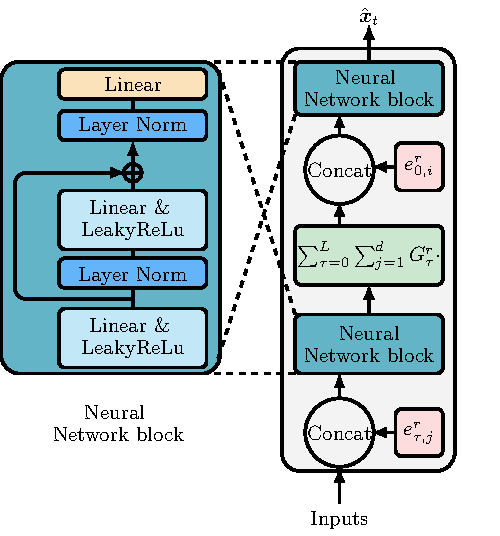
\includegraphics[width=0.4\textwidth]{figures/Fantom_TGNN_tikz.pdf}
  \end{center}
  \vspace{-10pt}
  \caption{Temporal graph neural network (TGNN) used by FANTOM.}
  \vspace{-5pt}
  \label{archi_fantom_tgnn}
\end{wrapfigure}
where $\psi^r$ and $\vartheta^r$ are neural network blocks illustrated in Figure \ref{archi_fantom_tgnn} with all the other colored blocks. Instead of using a neural network block per node, we adopt a weight-sharing mechanism by using a trainable embeddings $e_{\tau,i}$ for $\tau \in [|0:L|]$ and $i \in \{1, \cdots, d\}$. For the heteroscedastic term, we introduce an invertible mapping  $ \ell^{i,r}_{\theta^r}: \mathbb{R} \rightarrow \mathbb{R}$ such that:
$$\ell^{i,r}_{\theta^r} \left(g^{i,r}\left(\mathbf{P a}_{\mathcal{G}^r}^i(<t), \mathbf{P a}_{\mathcal{G}^r}^i(t)\right)\cdot\epsilon_t^{i,r}\right) = n^{i,r}_t,$$ where $n^{i,r}_t \sim \mathcal{N}(0,1)$. The design of $\ell^{i,r}_{\theta^r}$ needs to properly balance the flexibility and tractability of the transformed noise density. We choose a conditional normalizing flows, for heteroscedastic noise, called conditional spline flow \citep{durkan2019neural}, that transforms our heteroscedastic noise distribution to a fixed normal noise $n^{i,r}_t$ for regime $r$. The spline parameters are predicted using a hyper-network with a similar form as Eq.(\ref{neural_sem_archi}) to incorporate heteroscedasticity. Due to the invertibility of $\ell^{i,r}_{\theta^r}$, the noise likelihood conditioned on all parents is:
\begin{equation}
   \scalebox{1}{$p_{\text{hetero}}\left(g^{i,r}\left(\mathbf{P a}_{\mathcal{G}^r}^i(<t), \mathbf{P a}_{\mathcal{G}^r}^i(t)\right)\cdot\epsilon_t^{i,r}\mid \mathbf{P a}_{\mathcal{G}^r}^i(<t), \mathbf{P a}_{\mathcal{G}^r}^i(t)\right)=p_{n^{i,r}}\left(n_t^{i,r}\right)\left|\frac{\partial \ell^{i,r}_{\theta^r}}{\partial \epsilon_t^{i,r}}\right|$} ,
   \label{eq_condtion_NF}
\end{equation}
where \(p_{n^{i,r}}(\cdot)\) is the standard normal density. In the non-Gaussian, \emph{non-heteroscedastic} case, FANTOM learns a base distribution based on a composite affine-spline transformation of a standard Gaussian. Finally, the system parameters comprise the learnable parameters of the time varying weights $ \boldsymbol{\omega}^r$, of the variational inference $\phi^r$ and of the neural networks $\theta^r$. We use $\Theta$, introduced in Eq.(\ref{elbo_eq}), to note all the learnable parameters of FANTOM, and we have the set of parameters is: $
\Theta=\left\{\left(\boldsymbol{\omega}^r, \phi^r, \theta^r\right)\right\}_{r=1}^{N_w} .
$
\subsection{BEM algorithm}
\subsubsection{M step: graph learning}
\label{sec_Mstep}
FANTOM applies BEM to maximize the ELBO described in Proposition \ref{elbo_eq}. It begins by initializing the regime partitions $\beta^r_{t} = p( z_t = r  | \boldsymbol{x}_t, \boldsymbol{x}_{<t})$ using equally sized windows, selected via a hyperparameter. Note that these binary regime indices $\beta^r_{t}$ are updated during the E-step. Then, in the M-step, FANTOM incorporates $\beta^r_{t}$ in the ELBO Eq.(\ref{elbo_eq}) to estimate the DAGs for each regime and learn the parameters $\boldsymbol{\omega}^r$ that align $\pi_t(\boldsymbol{\omega}^{r})$ with $\beta^r_{t}$. We have:

\begin{equation}
\begin{aligned}
       \argmaxA_{\Theta}&  \Big\{\color{teal}\mathbb{E}_{q_\phi\left(\mathcal{G}\right)}\left[\sum_{t=1}^{|\mathcal{T}|} \sum_{r=1}^{N_w}\beta^r_{t}\log p_{\theta_{r}}\left(\boldsymbol{x}_t\mid \boldsymbol{x}_{<t}, \mathcal{G}^{r}\right)\right]+\sum_{r=1}^{N_w} \mathbb{E}_{q_{\phi_r}\left(\mathcal{G}^r\right)}\left[\log p\left(\mathcal{G}^r\right)\right]+H\left(q_{\phi_r}\left(\mathcal{G}^r\right)\right)\\
       &+ \color{cyan}\sum_{t=1}^{|\mathcal{T}|} \sum_{r=1}^{N_w}\beta^r_{t}\log \pi_t(\boldsymbol{\omega}^{r})\color{black}\Big\},
\end{aligned}
\label{Mstep_eq_colored}
\end{equation}
The maximization of the above equation can be decomposed into two distinct and separate maximization problems. The first problem, \textcolor{cyan}{regime alignment}, focuses on aligning $\pi_t(\boldsymbol{\omega}^{r})$ with $\beta^r_{t}$. While the second one, \textcolor{teal}{graph learning}, involves estimating DAGs for every regime.\\
For the graph prior $p\left(\mathcal{G}^r\right)$ for all $r \in [|1:N_w|]$ have to combine two components: DAG constraint and graph sparseness prior. Inspired by \citep{zheng2018dags, gong2022rhino, geffner2022deep}, we propose the following unnormalised prior $
p\left(\mathcal{G}^r\right) \propto \exp \left(-\lambda_s\left\|\boldsymbol{G}^r_{0: K}\right\|_F^2-\rho h^2\left(\boldsymbol{G}^r_0\right)-\alpha h\left(\boldsymbol{G}^r_0\right)\right).
$ Using Eq.(\ref{proba_nf_math}), we have
$
     \log p_{\theta^{r}}\left(\boldsymbol{x}_t\mid \boldsymbol{x}_{<t}, \mathcal{G}^{r}\right)= \sum_{i=1}^{d} \log p_{\text{hetero}}\left(y_t^{i,r} \mid \mathbf{P a}_{\mathcal{G}^r}^i(<t), \mathbf{P a}_{\mathcal{G}^r}^i(t)\right),
$ where $p_{\text{hetero}}$ and $y_t^{i,r}$ are defined in Eq.(\ref{eq_condtion_NF}). The parameters $\theta^r, \phi^r$ are learned by maximizing the \textcolor{teal}{graph learning} maximization problem Eq.(\ref{Mstep_eq_colored}), where the Gumbel-softmax gradient estimator is used \citep{jang2016categorical}. We also leverage augmented Lagrangian
training similar to \citep{pamfil2020dynotears, rahmanicausal, geffner2022deep}, to anneal $\alpha, \rho$.
\subsection{E step: Regime learning}
\label{sec_Estep}
In the E-step, FANTOM updates the posterior probability $\beta^r_{t} = p( z_t = r  | \boldsymbol{x}_t, \boldsymbol{x}_{<t})$ (see Eq.(\ref{10}), with derivation provided in Appendix \ref{Estep_illustration}):
\begin{equation}
\begin{aligned}
\textcolor{black}{\beta^r_{t}} & \textcolor{black}{=\frac{p\left(z_{t}=r\right) p\left(\boldsymbol{x}_t \mid \boldsymbol{x}_{<t}, z_{t}=r, \mathcal{G}^r\right)}{\sum_{j=1}^{N_w} p\left(z_{t}=j\right) p\left(\boldsymbol{x}_t \mid \boldsymbol{x}_{<t}, z_{t}=j, \mathcal{G}^j\right)}} \\
& \textcolor{black}{\propto \pi_t(\boldsymbol{\omega}^{r}) p\left(\boldsymbol{x}_t \mid \boldsymbol{x}_{<t}, z_{t}=r, \mathcal{G}^r\right)},
\end{aligned}
\label{10}
\end{equation}
where $p(\boldsymbol{x}_t \mid \boldsymbol{x}_{<t}, z_{t} = r, \mathcal{G}^r)$ denotes the observational likelihood of $\boldsymbol{x}_t$ being generated by the SEM from Eq~(\ref{eq_multi_reg_hetero}) for regime $r$. This probability is computed using the CNFs trained during the M-step, following the same reasoning as in Eq.(\ref{proba_nf_math}).

\begin{wrapfigure}{r}{0.45\textwidth}
\begin{center}
    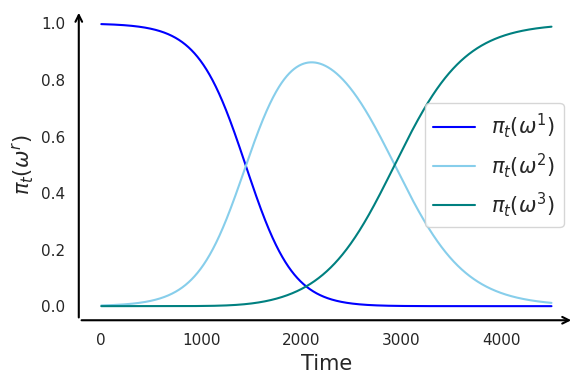
\includegraphics[width=0.45\textwidth]{figures/alignement_plot.png}
  \end{center}
  \vspace{-10pt}
  \caption{Illustration of $\pi_t\left(\boldsymbol{\omega}^r\right)$ after Fantom's first iteration with equal windows of 1500 samples for an MTS of 4500 samples with two ground-truth regimes: $\mathcal{I}^{*}_1 = [|0:1999|]$ and $\mathcal{I}^{*}_2 = [|2000:4500|]$.}
  \label{fig:pi_alignement}
  \vspace{-5pt}
\end{wrapfigure}
The probability of $\boldsymbol{x}_t$ belonging to regime $r$ is influenced by two main factors: the observation’s position within its current regime and whether that regime is designated as \textcolor{RoyalBlue}{pure or impure}.
For example, if $\boldsymbol{x}_t$ is in a \textcolor{RoyalBlue}{pure} regime $r$ but is near the boundary in the current iteration, $\pi_t(\boldsymbol{\omega}^r)$ and $\pi_t(\boldsymbol{\omega}^{r+1})$ are nearly equal (e.g., $\pi_{t \in [1100,1500]}(\boldsymbol{\omega}^1)$ vs.\ $\pi_{t \in [1100,1500]}(\boldsymbol{\omega}^2)$ in Figure~\ref{fig:pi_alignement}). Nonetheless, since regime $r$ was learned from pure data, $p(\boldsymbol{x}_t \mid \boldsymbol{x}_{<t}, z_t = r, \mathcal{G}^r)$ stays high, keeping $\beta_t^r$ at its maximum value and maintaining $\boldsymbol{x}_t$ in regime $r$ for the next iteration. In the other hand, if $\boldsymbol{x}_t$ is in an \textcolor{RoyalBlue}{impure} regime $r+1$ near the boundary during the current iteration, $\pi_t(\boldsymbol{\omega}^r)$ and $\pi_t(\boldsymbol{\omega}^{r+1})$ are also close in value (e.g., $\pi_{t \in [1501,1800]}(\boldsymbol{\omega}^1)$ vs.\ $\pi_{t \in [1501,1800]}(\boldsymbol{\omega}^2)$ in Figure \ref{fig:pi_alignement}). However, because the causal graph for regime $r$ is more reliable (having been derived from pure data),
$
p(\boldsymbol{x}_t \mid \boldsymbol{x}_{<t}, z_t = r, \mathcal{G}^r)
>
p(\boldsymbol{x}_t \mid  \boldsymbol{x}_{<t}, z_t = r+1, \mathcal{G}^{r+1}).
$
As a result, $\boldsymbol{x}_t$ moves from regime $r+1$ to $r$ in the next iteration.
%\textbf{Case 4:}
%$\boldsymbol{x}_t$ belongs to impure regime $r+1$ and is far from the border (e.g., $t \in [1700,2000]$ in Figure \ref{fig:pi_alignement}). In this case, it's uncertain whether $\boldsymbol{x}_t$ will switch regimes in the next iteration. However, as the pure regime $r$ expands with each iteration, $\boldsymbol{x}_t$ will eventually be near the border of regime $r+1$, bringing us back to Case~3.
For simplicity reasons, we explicit these cases from one border but the same thing happens in the other border which accelerates convergence. More details about other cases and Figures that illustrate the idea could be found in Appendix \ref{Estep_illustration}. 

After updating $\beta^r_{t}$, for each sample $\boldsymbol{x}_t$, FANTOM assigns a value of 1 to the most probable regime $r$ (with the highest $\beta^r_{t}$), and 0 to others. Additionally, FANTOM filters out regimes with insufficient samples (fewer than $\zeta$, the minimum regime duration, defined as a hyper-parameter). Discarded regime samples are then reassigned to the nearest regime in terms of probability $\beta^r_{t}$ in the subsequent iteration which is in general a neighboring regime ensured by the way we set up the probability $\beta^r_{t}\propto \pi_t(\boldsymbol{\omega}^{r}) p\left(\boldsymbol{x}_t \mid \boldsymbol{x}_{<t}, z_{t}=r, \mathcal{G}^r\right)$.